% The generic preamble
\documentclass[10pt,letterpaper,fleqn,titlepage]{article}

% Define packages to use
\usepackage{natbib}
\usepackage[dvips]{graphicx,color}
\usepackage{amsmath,amssymb}
\usepackage{bm}
\usepackage{caption}
\usepackage{xr}
\usepackage{ifthen}
\usepackage[dvipdfm,colorlinks,linkcolor=blue,citecolor=blue,urlcolor=blue]{hyperref}
\usepackage{fancybox}
\usepackage{textcomp}
\usepackage{alltt}
%\usepackage{floatflt}
%\usepackage{svn}


% Redefine default page
\setlength{\textheight}{9in}  % 1" above and below
\setlength{\textwidth}{6.75in}   % 0.5" left and right
\setlength{\oddsidemargin}{-0.25in}

% Redefine default paragraph
\setlength{\parindent}{0pt}
\setlength{\parskip}{1ex plus 0.5ex minus 0.2ex}

% Define caption width and default fonts
\setlength{\captionmargin}{0.5in}
\renewcommand{\captionfont}{\sffamily}
\renewcommand{\captionlabelfont}{\bfseries\sffamily}

% Define commands for super- and subscript in text mode
\newcommand{\superscript}[1]{\ensuremath{^\textrm{#1}}}
\newcommand{\subscript}[1]{\ensuremath{_\textrm{#1}}}

% Derived commands
\newcommand{\invcm}{\textrm{cm\superscript{-1}}}
\newcommand{\micron}{\ensuremath{\mu\textrm{m}}}

\newcommand{\df}{\ensuremath{\delta f}}
\newcommand{\Df}{\ensuremath{\Delta f}}
\newcommand{\dx}{\ensuremath{\delta x}}
\newcommand{\Dx}{\ensuremath{X_{max}}}
\newcommand{\Xeff}{\ensuremath{X_{eff}}}

\newcommand{\water}{\textrm{H\subscript{2}O}}
\newcommand{\carbondioxide}{\textrm{CO\subscript{2}}}
\newcommand{\ozone}{\textrm{O\subscript{3}}}

\newcommand{\taup}[1]{\ensuremath{\tau_{#1}}}
\newcommand{\efftaup}[1]{\ensuremath{\tau_{#1}^{*}}}

\newcommand{\textbfm}[1]{\boldmath\ensuremath{#1}\unboldmath}

\newcommand{\rb}[1]{\raisebox{1.5ex}[0pt]{#1}}

\newcommand{\f}[1]{\texttt{#1}}

% Define how equations are numbered
\numberwithin{equation}{section}
\numberwithin{figure}{section}
\numberwithin{table}{section}

% Define a command for title page author email footnote
\newcommand{\email}[1]
{%
  \renewcommand{\thefootnote}{\alph{footnote}}%
  \footnote{#1}
  \renewcommand{\thefootnote}{\arabic{footnote}}
}

% Define a command to print the Office Note subheading
\newcommand{\notesubheading}[1]
{%
  \ifthenelse{\equal{#1}{}}{}
  { {\Large\bfseries Office Note #1\par}%
    {\scriptsize \sc This is an unreviewed manuscript, primarily intended for informal}\\ 
    {\scriptsize \sc exchange of information among JCSDA researchers\par}%
  }
}

% Redefine the maketitle macro
\makeatletter
\def\docseries#1{\def\@docseries{#1}}
\def\docnumber#1{\def\@docnumber{#1}}
\renewcommand{\maketitle}
{%
  \thispagestyle{empty}
  \vspace*{1in}
  \begin{center}%
     \sffamily
     {\huge\bfseries Joint Center for Satellite Data Assimilation\par}%
     \notesubheading{\@docnumber}
  \end{center}
  \begin{flushleft}%
     \sffamily
     \vspace*{0.5in}
     {\Large\bfseries\ifthenelse{\equal{\@docseries}{}}{}{\@docseries: }\@title\par}%
     \medskip
     {\large\@author\par}%
     \medskip
     {\large\@date\par}%
     \bigskip\hrule\vspace*{2pc}%
  \end{flushleft}%
  \newpage
  \setcounter{footnote}{0}
}
\makeatother
\docseries{}
\docnumber{}


% Define a command for a DRAFT watermark
\usepackage{eso-pic}
\newcommand{\draftwatermark}
{
  \AddToShipoutPicture{%
    \definecolor{lightgray}{gray}{.85}
    \setlength{\unitlength}{1in}
    \put(2.5,3.5){%
      \rotatebox{45}{%
        \resizebox{4in}{1in}{%
          \textsf{\textcolor{lightgray}{DRAFT}}
        }
      }
    }
  }
}




% Title info
\title{Analyzing Zeeman Impact On Upper Atmosphere Sounding Channels Using a Zeeman Turned Off LBL Model as Reference}
\author{David Neil Groff}
\date{01/17/07}

\newcommand{\microtesla}{\ensuremath{\mu\textrm{T}}}
%-------------------------------------------------------------------------------
%                            Ze document begins...
%-------------------------------------------------------------------------------
\begin{document}
\maketitle

\section{Introduction}
%=================
Special Sensor Microwave Imager/Sounder (SSMIS) upper atmosphere sounding channels 19-22 are significantly affected
by Zeeman splitting \cite{ref:Han1}. Taking into account the Zeeman Effect in RT models has been
shown to significantly improve observation versus model brightness temperature
residuals for high peaking SSMIS channels 19-21 [Han et al., 2007].
This report is concerned with brightness temperature (BT) comparisons between two models that
account for Zeeman splitting and a reference model
that does not account for Zeeman splitting. Comparisons are performed for SSMIS channels 19-24.
The motivation of this report is to 
determine to what extent the aforementioned comparisons
are qualititatively consistent with a reasoned explanation of how Zeeman splitting 
should impact measured BT's for SSMIS channels 19-21.
    
\subsection{No Zeeman Model}
BT calculations for Liebe model transmittances that do not account for Zeeman splitting serve
as a "Zeeman turned off" reference in this report. BT's calculated from Liebe and
Rosenkranz transmittances that do not account for Zeeman splitting agree to within 0.1K for SSMIS channels 19-24 as shown in Figure 1.  
These differences are small compared to the absolute impact of Zeeman splitting for SSMIS channels 19-21. Therefore, it is reasonable to use
either "Zeeman turned off" model as a reference when comparing against the "Zeeman turned on"
models considered in this paper. 

%-----------------------
. 

\begin{figure}[htp]
  \centering{}
  \includegraphics[scale=0.8]{./graphics/Rosenkranz_V_Liebe.eps}
  \caption[below]{Comparison of brightness temperatures between Rosenkranz and Liebe models which do not account for Zeeman splitting.}
  \label{fig:Rosenkranz_V_Liebe}
\end{figure}

\newpage
\section{Zeeman Splitting Effects}

Channels 19 and 20 have weighting functions that peak in the mesosphere. These channels are centered on O\subscript{2} rotational absorption
lines. As explained in [Han et al., 2007] Zeeman splitting of O\subscript{2} absorption lines decreases the altitude at which the weighting functions for these channels
peak. This is because the passbands for channels 19 and 20 are centered on O\subscript{2} rotational transition lines [Han et al., 2007]. Conversely, 
Zeeman splitting increases the altitude at which the weighting function for channel 21 peaks, because the channel is slightly offset from the O\subscript{2} 
transition line. Figure 2 demonstrates the relationship between increased Zeeman splitting and the peak 
weighting function altitudes for channels 19-21. All three channels peak in the mesosphere where lapse rates are normally negative. Therefore, Zeeman splitting should cause an increase in 
observed brightness temperatures for channels 19 and 20, but a decrease in observed brightness temperatures for channel 21. Figure 2 also demonstrates 
that the impact of Zeeman splitting is related to the view angle with respect to the geomagnetic field.

\begin{figure}[htp]
  \centering{}
  \includegraphics[scale=0.8]{./graphics/Figure2.eps}
  \caption{(A) Weighting functions calculated with B=23\microtesla{} (solid lines) and B=60\microtesla{} (dashed lines) and (B) with theta=0 (solid lines) and theta=90 (dashed lines)
  at B=60\microtesla{} (Where theta is the angle between the view direction and the geomagnetic field).}
  %\label{fig:blah_ref2}
\end{figure}

\newpage
\section{Liebe "Zeeman On" Versus Liebe "Zeeman Off"}
The Liebe model that takes into account Zeeman splitting assumes a fixed magnetic field
for all simulations (B = 60\microtesla{}). Figure 3 shows comparisons between Liebe "Zeeman turned
on" BT's and Liebe "Zeeman turned off" BT's. The sign and shape of the differences for channels 19-21 appear to be reasonably consistent 
with the impact of Zeeman splitting descibed in [Han et. al, 2007] and with a reasoned argument
for Zeeman splitting effects on BT's for these channels. However, the magnitudes of the differences for channels 19 and 20 are more than a factor of 
two smaller than the magnitude of the difference for channel 21. 
 
\begin{figure}[htp]
  \centering{}
  \includegraphics[scale=0.8]{./graphics/Liebe_Comparison.eps}
  \caption{(A) Weighting functions calculated with B=23\microtesla{} (solid lines) and B=60\microtesla{} (dashed lines) and (B) with theta=0 (solid lines) and theta=90 (dashed lines)
  at B=60\microtesla{} (Where theta is the angle between the view direction and the geomagnetic field).}
  %\label{fig:blah_ref2}
\end{figure}
 
This result is not consistent with calculations using the fast RT model [Han et. al., 2007].
In Figure 4 the impact of Zeeman splitting as a function of magnetic field strength is plotted for 11 different view geometries with respect to the geomagnetic
field. For the plots in Figure 4 all differences/offsets are relative to BT's calculated for a base magnetic field strength of 20\microtesla{}. At all view
geometries with respect to the geomagnetic field the absolute magnitudes of the differences/offsets for channels 19 and 20 are similar to the absolute
magnitude of the difference/offset for channel 21.   

\newpage

\begin{figure}[htp]
  \centering{}
  \includegraphics[scale=0.8]{./graphics/Figure4.eps}
  \caption{Brightness temperatures as a function of the geomagnetic field strength for 11 view geometries with
   respect to the geomagnetic field.}
  %\label{fig:blah_ref2}
\end{figure}

\section{Fast RT Model "Accounting For Zeeman Effect" Versus Liebe "Zeeman Turned Off" Comparisons}
The fast model that accounts for the Zeeman Effect was trained by a data set prepared
at zenith angles confined between 51-54 degrees (Scan angle fixed at 45), 11 points on (20<B<70)
and 6 points on cos(Theta) (0<theta<90). The inputs for the fast model are layer temperature, the cosine
of the view geometry with respect to the geomagnetic field and magnetic field strength. The model outputs 
brightness temperatures for channels 19-24 at a zenith angle of approximately 52.5 degrees. 

Example results are included in the tarball package for this model. 
To confirm that I was appropriately using the model I reproduced 
the example result brightness temperatures.

Figure \ref{fig:xx} shows mean brightness temperature differences between the fast RT model and the Reference model for 
magnetic fields of 23\microtesla{} and 60\microtesla{}. The sign of the differences and the absolute magnitude
of the differences in Figure 5 are not consistent with relative changes/offsets shown in the Figure 4 plots. However,
the Figure 4 plots are relative to a calculation that accounts for the Zeeman Effect given a magnetic field of 20\microtesla{}
Furthermore as the magnetic field is increased the fast RT model BT's are more similar to the Liebe "Zeeman turned
off" BT's for channels 19 and 20. As the magnetic field increases the impact of the Zeeman splitting on BT's should
increase. 
   
\begin{figure}[htp]
  \centering{}
  \includegraphics[scale=0.8]{./graphics/Figure5.eps}
  \caption{Mean differences between a fast RT model that accounts for the Zeeman Effect and a reference "Zeeman turned off"
   model. The differences were calculated for magnetic fields of 23\microtesla{} and 60\microtesla{}}
  \label{fig:xx}
\end{figure}


%Stuff is shown in figure \ref{fig:blah_ref} ...




\newpage
%=================


%\begin{table}[htp]
 % \centering
  %\begin{tabular}{c | c}
  %  Col1 & Col2\\
  %  \hline
  %  1 & a\\
  %  2 & b\\
  %  3 & c
  %\end{tabular}
  %\caption{Caption for blah table}
  %\label{tab:blah_ref}
%\end{table}



\begin{figure}[htp]
  \centering
  %\includegraphics{2006jd008208_f01_orig.eps}
  \caption{Caption for blah}
  \label{fig:blah_ref}
\end{figure}



% The references section
%=======================
\begin{thebibliography}{99}
  \bibitem{ref:Han1} reference for Yongs paper
  \bibitem{ref:tag2} reference2
\end{thebibliography}



% The appendices section
%=======================
\begin{appendix}
\end{appendix}


\end{document}

